\documentclass[9pt,dvipsnames]{beamer}
\usepackage[T1]{fontenc}
\usepackage{libertinus}
\usepackage{amsmath}
\usepackage[most]{tcolorbox}
\usepackage{pgfplots}
\usepackage{graphicx}

\usepackage{hyperref}

\usepackage{xcolor}  
\newcommand{\cb}[1]{{\color{CadetBlue}#1}}


\usetheme{Berkeley}
\setbeamertemplate{navigation symbols}{}


\title{CSE574 Introduction to Machine Learning}
\subtitle{Support Vector Machine}
\author{Jue Guo}
\institute{University at Buffalo}
\date{\today}

\begin{document}
\begin{frame}
	\titlepage
\end{frame}

\begin{frame}
	\frametitle{Outline}
	\tableofcontents
\end{frame}
\section{Alternative View of Logistic Regression}
\begin{frame}{Alternative View of Logistic Regression}
	\begin{columns}
		\column{0.5\textwidth}
		A quick review: $h_\theta(x)=\frac{1}{1+e^{-\theta^T x}}$
		\begin{itemize}
			\item if \(y=1\), we want $h_\theta(x) \approx 1$, $\theta^T x \gg 0$
			\item if \(y=0\), we want \(h_\theta(x) \approx 0\), $\theta^T x \ll 0$
		\end{itemize}
		\column{0.5\textwidth}
		\begin{figure}
			\centering
			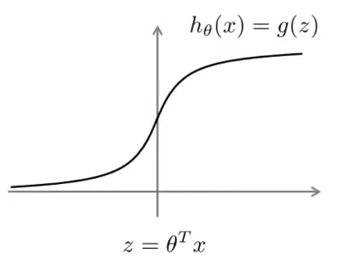
\includegraphics[width=0.9\textwidth]{imgs/svm_1.png}
		\end{figure}

	\end{columns}
	The cost of a single example:

	\begin{align*}
		  & -\left(y \log h_\theta(x)+(1-y) \log \left(1-h_\theta(x)\right)\right)                    \\
		= & -y \log \frac{1}{1+e^{-\theta^T x}}-(1-y) \log \left(1-\frac{1}{1+e^{-\theta^T x}}\right)
	\end{align*}
\end{frame}

\begin{frame}
	\[
		-y \log \frac{1}{1+e^{-\theta^T x}}-(1-y) \log \left(1-\frac{1}{1+e^{-\theta^T x}}\right)
	\]
	\begin{columns}
		\column{0.5\textwidth}
		if \(y=1\) (want $\theta^T x \gg 0$)
		\begin{figure}
			\centering
			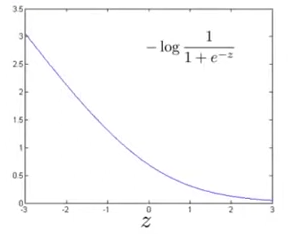
\includegraphics[width=0.7\textwidth]{imgs/svm_2.png}
		\end{figure}
		\column{0.5\textwidth}
		if \(y=0\) (want $\theta^T x \ll 0$)
		\begin{figure}
			\centering
			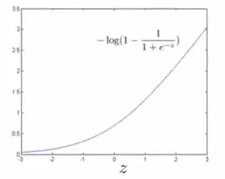
\includegraphics[width=0.7\textwidth]{imgs/svm_3.png}
		\end{figure}
	\end{columns}
\end{frame}

\section{Support Vector Machine}
\begin{frame}{Support Vector Machine}
	\textbf{Cost Function of Logistic Regression}
	\begin{align*}
		\min _\theta \frac{1}{m}\Bigg[ & \sum_{i=1}^m y^{(i)}\left(-\log h_\theta\left(x^{(i)}\right)\right)                          \\
		                               & + \left(1-y^{(i)}\right)\left(-\log \left(1-h_\theta\left(x^{(i)}\right)\right)\right)\Bigg] \\
		                               & + \frac{\lambda}{2 m} \sum_{j=1}^n \theta_j^2
	\end{align*}
	\textbf{Cost Function of Support Vector Machine}
	$$
		\min _\theta C \sum_{i=1}^m\left[y^{(i)} \operatorname{cost}_1\left(\theta^T x^{(i)}\right)+\left(1-y^{(i)}\right) \operatorname{cost}_0\left(\theta^T x^{(i)}\right)\right]+\frac{1}{2} \sum_{i=1}^n \theta_j^2
	$$
\end{frame}

\begin{frame}{Large Margin Intuition}
	\textbf{Support Vector Machine}
	$$
		\min _\theta C \sum_{i=1}^m\left[y^{(i)} \operatorname{cost}_1\left(\theta^T x^{(i)}\right)+\left(1-y^{(i)}\right) \operatorname{cost}_0\left(\theta^T x^{(i)}\right)\right]+\frac{1}{2} \sum_{i=1}^n \theta_j^2
	$$
	\begin{tikzpicture}[scale=0.7]
		\begin{axis}[
				axis lines=middle,
				axis line style={->},
				xlabel={$z$},
				ylabel={},
				xlabel style={at={(ticklabel* cs:1)},anchor=north west},
				ylabel style={at={(ticklabel* cs:1)},anchor=south west},
				xtick={-1,1},
				ytick={0,1},
				ymin=-0.5, ymax=1.5,
				xmin=-1.5, xmax=1.5,
				clip=false,
				width=10cm,
				height=5cm,
				ticks=none
			]

			% Add the line plot for z < 1
			\addplot[domain=-1.5:1, samples=2, thick] {-x+1};
			% Add the horizontal line plot for z >= 1
			\addplot[domain=1:1.5, samples=2, thick] {0};

		\end{axis}
	\end{tikzpicture}
\end{frame}

\begin{frame}
	\begin{center}
		\Huge Questions?
	\end{center}
\end{frame}
\end{document}